\newpage
\section{ Árboles de decisión y bosques aleatorios}

\noindent Sea un vector aleatorio $\textbf{x}$ de longitud $p$ con las variables predictoras e $Y$ la variable respuesta. Se toman $N$ observaciones obteniéndose parejas $(\textbf{x}_i,y_i)$. De esta manera, tenemos que se puede interpretar que $\mathbf{x}_i\in\mathbb{R}^p$.

\noindent Los árboles de decisión son métodos divisivos que fragmentan  el espacio de observaciones $\mathbb{R}^p$ en varias regiones. En cada región, se ajusta un modelo más simple.

\noindent La ventaja de este tipo de métodos es que son fácilmente interpretables, ya que pueden ser representados mediante un diagrama de tipo árbol. De esta manera, entre los principales objetivos de los árboles de decisión, se encuentran la selección y evaluación de la importancia de las variables \cite{Brown 2004,Song 2015}. Además se pueden utilizar con fines predictivos o incluso de manejo de los datos, valores perdidos entre otros \cite{Nerini 2007}.

\noindent Otra ventaja de este tipo de métodos es que permite trabajar con conjuntos de datos en los que se estudian un mayor número de variables que de observaciones, es decir, $p > N$ \cite{Diaz 2006}. 

\noindent El problema que más se da en los árboles de decisión es su tendencia al sobreajuste, ya que de la forma que están conceptualizados, provoca que el sesgo sea pequeño, pero con una gran varianza. Esto se considera en los algoritmos desarrollados durante la sección, normalmente se eliminan particiones que no aporten demasiado. A este proceso se le llama ``poda". Es por esta problemática que se desarrolla el análisis de modelos mediante la descomposición en sesgo y varianza de los mismos. 

\noindent Se detallan los principales conceptos y notación a continuación. 

\subsection{Conceptos básicos}
\noindent Para empezar hay que definir el concepto inicial de un árbol de decisión \cite{Hastie 2001}.
\begin{defi}
Un árbol de decisión es un conjunto de reglas discriminantes que fraccionan el espacio de observaciones de acuerdo a un cierto criterio. Este conjunto genera un grafo de tipo árbol con un único nodo raíz  y donde los nodos hoja representan cada una de las regiones en las que se ha fraccionado el espacio. 
\end{defi}
\noindent Como se ha dicho un árbol de decisión genera particiones del espacio de observaciones que se definen de la siguiente manera \cite{Brown 2004}.
\begin{defi}
Se llama separación, partición o división de índice $(j,s)$ a la fragmentación del espacio inicial dado en las siguientes regiones $R_1,R_2$:
\begin{equation}
R_1=\lbrace \mathbf{x}_i \in \mathbb{R}^p/ x_{ij}>s\rbrace \quad R_2=\lbrace \mathbf{x}_i \in \mathbb{R}^p/ x_{ij}\leq s\rbrace
\end{equation}

\noindent Hay que tener en cuenta que esto sería en el caso en el que la variable a separar $X_j$ sea continua.

\noindent En el caso de que la variable a particionar sea categórica o cualitativa Breiman propone la siguiente solución \cite{Breiman 1984}. Supongamos que $X_j$ toma $L$ valores distintos en un nodo en específico. Entonces podemos tomar un conjunto de valores $L_1\subset L$ de tal manera que las regiones que se obtienen son:
\begin{equation}
R_1=\lbrace \mathbf{x}_i \in \mathbb{R}^p/ x_{ij}=l/ l\in L_1\rbrace \quad R_2=\lbrace \mathbf{x}_i \in \mathbb{R}^p/ x_{ij}=l/ l\notin L_1\rbrace
\end{equation}
\end{defi}
\begin{defi}
Se define como nodo de un árbol de decisión, a cada una de las regiones resultantes después de aplicar una separación.
\end{defi}
\noindent En particular se tienen los nodos terminales o hoja y los nodos padre y nodos hijo \cite{Brown 2004}.
\begin{defi}
Se define un nodo terminal o nodo hoja en un árbol de decisión como cada una de las regiones finales resultante de la partición del espacio de observaciones.
\end{defi}
\begin{defi}
Se denomina nodo padre al nodo previo a una  separación y se definen los nodos hijos a los resultantes de dicha partición. 
\end{defi}
\noindent Además podemos dar varias medidas de la complejidad del modelo \cite{Hastie 2001}.
\begin{defi}
Se denomina  tamaño del árbol $T$, $|T|$ al número de nodos terminales. 
\end{defi}
\begin{defi}
Se llama profundidad del árbol al número máximo de divisiones necesarias para llegar a un nodo terminal. 
\end{defi}
\noindent Las  siguientes imágenes \ref{f:diagrama arbol}, \ref{f:división}  muestran el diagrama resultante tras dividir el espacio de observaciones mediante un árbol. 

\begin{figure}[h]
 \centering
  \subfloat[División de $\mathbb{R}^p$]{
   \label{f:división}
    \includegraphics[width=0.4\textwidth]{Documentos Extra/Imagenes/Regiones árboles.png}}
  \subfloat[Diagrama resultante]{
   \label{f:diagrama arbol}
    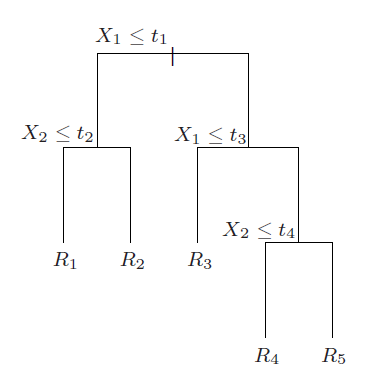
\includegraphics[width=0.4\textwidth]{Documentos Extra/Imagenes/Diagrama de arbol.png}}
 \caption{Representación de la división de $\mathbb{R}^p$ y el diagrama de árbol resultante.Ambas procedentes de \cite{Hastie 2001}.}
 \label{f:MARC1}
\end{figure}

\noindent Como se puede ver, cada uno de los nodos terminales representa cada una de las regiones en las que se ha separado el espacio de observaciones. 

\noindent Dependiendo del tipo de variable respuesta, se utiliza un árbol de regresión cuando se busca estudiar la relación de un conjunto de variables con otra variable continua, y un árbol de clasificación cuando la variable respuesta es categórica o cualitativa. En nuestro caso, los algoritmos que se describirán pueden manejar tanto variables de entrada discretas como continuas. Se detallará a continuación el caso en el que las variables de entrada son continuas.

\noindent \emph{Observación:} se usan particiones binarias porque son simples de comprender y manejar. Esto facilita el uso de árboles de decisión y nos ayuda a entender las áreas que creamos al dividir los datos.

%\noindent Esta parte se va utilizar, tanto en los árboles como en los random forests, ya que son métodos que buscan con un conjunto relativamente pequeño de observaciones en relación con el numero de variables observadas obtener un modelo que no tenga un sobreajuste excesivo. De hecho, para hacer crecer un árbol, se busca hacerlo crecer hasta un punto de sobreajuste y luego se irá ``podando" de la manera que se definirá más tarde para evitar dicho sobreajuste introduciendo algo de sesgo. 

\subsection{Árboles de regresión }
\noindent A continuación, examinemos el  proceso de crecimiento de un árbol de regresión. Se considera un vector aleatorio $\mathbf{x}$ con $p$ variables predictoras y una variable respuesta continua $Y$. Aunque hay varios algoritmos para hacer crecer los árboles de regresión se detallará el algoritmo \emph{CART} (árboles de clasificación y regresión) de Breiman \cite{Breiman 1984}. Se elige este ya que es el más importante y fundamental. 

\noindent Supongamos que hemos establecido un número máximo de particiones $M=|T|$. El objetivo del árbol de regresión es dividir el espacio de observaciones en regiones $R_m$ para $m=1,\ldots, M$. Cada región $R_m$ está asociada a su función característica, que denotaremos como $\mathbf{1}_m$.

\noindent En el caso de que se tomen $N$ observaciones, podemos definir el estimador resultante $\hat{f}(\mathbf{x})$ de la siguiente manera:

\begin{equation}
\hat{f}(\mathbf{x})=\sum_{m=1}^M \hat{f}_m(\mathbf{x})\cdot \mathbf{1}_m(\mathbf{x})
\end{equation}

\noindent Esto significa que en cada región $R_m$, se realiza una regresión utilizando los datos correspondientes a esa región. Generalmente, se busca una aproximación lo más sencilla posible en cada $R_m$, por ejemplo, utilizando una constante. \cite{Biau 2016,Hastie 2001}.

\noindent Si se aplica el método de los mínimos cuadrados, con la restricción requerida, se pueden definir las constantes $\hat{c}_m$ de la siguiente manera (Para ver demostración completa véase la sección de 9.1 \cite{Breiman 1984}):
\begin{equation}
\hat{c}_m=\dfrac{1}{N_m}\sum_{i/\mathbf{x}_i\in R_m} y_i
\end{equation}

\noindent Donde $N_m$ es el número de observaciones que hay en $R_m$. Es decir, $\hat{c}_m$ es la media muestral de las respuestas de las observaciones que pertenecen a la región y esto provoca que $\hat{f}(\mathbf{x})=\sum_{m=1}^M \hat{c}_m \cdot \mathbf{1}_m(\mathbf{x})$. Es decir, la predicción $\hat{y}$ para un $\mathbf{x}\in R_m$ otorgada por el modelo es $\hat{c}_m$ \cite{Hastie 2001, Breiman 1984}.

\noindent Una vez se conoce como se va a dar la estimación final, hay que saber cómo llegar a la mejor partición. Este proceso de selección puede cambiar de un algoritmo a otro.  

\noindent En regresión, hay que elegir $j$ y $s$ de tal manera que las regiones resultantes $R_{m_1},R_{m_2}$ de la partición $(j,s)$ son aquellas en las que se minimiza la siguiente expresión \cite{Breiman 1984}:
\begin{equation}
\sum_{i/\mathbf{x}_i\in R_{m_1} } (y_i-\hat{c}_{m_1})^2+\sum_{i/\mathbf{x}_i\in R_{m_2} } (y_i-\hat{c}_{m_2})^2
\end{equation}

\noindent Es decir, el objetivo es encontrar las separaciones que minimicen la suma de los errores cuadráticos. A este criterio se le llama \emph{CART}, aunque Biau y Scornet  lo plantean de manera distinta \cite{Biau 2016, Breiman 1984}. Podemos definir el error cuadrático medio de cada región de la siguiente manera \cite{Hastie 2001}.

\begin{defi}
Se llama error cuadrático medio de una región $R_m$ a $Q_m(T)=\frac{1}{N_m}\sum_{i/\mathbf{x}_i\in R_m}(y_i-\hat{c}_m)^2$ .
\end{defi}

\noindent Por tanto, podemos definir una función de coste general 
\begin{equation}
Q(T)=\sum_{m=1}^M\frac{1}{N_m}\sum_{i/\mathbf{x}_i\in R_m} (y_i-\hat{c}_m)^2,
\end{equation}


\noindent ya que el error cometido medio en el espacio de observaciones es la media de todos los errores cometidos en cada una de las regiones en las que se particiona el espacio \cite{Breiman 1984}. 

\noindent Por tanto, hacer crecer un árbol, es decir, hacer que tenga más nodos terminales, va a provocar que $N_m$ sea menor, por lo tanto, hacer crecer un árbol demasiado hace que estemos en un caso de sobreajuste, lo cual se desarrolla más adelante en esta sección. Es por ello, que se crean métodos como la poda.

\noindent Para empezar, hay que definir lo que significa la poda de un árbol. 
\begin{defi}
Se llama poda al proceso en el que dado un árbol inicial de tamaño $T_0$ se revierten ciertas particiones terminales que no aportan en la relación coste-complejidad, es decir, aumentan demasiado la complejidad (aumentando la varianza), sin reducir el coste en exceso. 
\end{defi}


\noindent Divakaran y Breiman proponen añadir un término al coste del árbol \cite{Breiman 1984,Divakaran 2022}. 
\begin{equation}
Q_{\alpha}(T)=\sum_{m=1}^M\frac{1}{N_m}\sum_{i/\mathbf{x}_i\in R_m} (y_i-\hat{c}_m)^2+\alpha|T |,
\end{equation}

\noindent donde $\alpha$ es un término para controlar la complejidad del árbol, es decir, $\alpha=0$ es el criterio habitual, mientras que cuanto mayor sea, más pequeños serán los árboles, ya que penaliza más el tamaño.  

\noindent El proceso que sugieren Divakaran, basado en el que da Breiman  viene dado por los siguientes pasos \cite{Breiman 1984,Divakaran 2022}:
\begin{itemize}
\item Primero prepara el conjunto de datos para poder realizar validación cruzada (Véase el Capítulo 7 de \cite{Hastie 2001}, en particular el método de \emph{K-folds}).

\item Se hace una partición binaria hasta tener un árbol de gran tamaño $T_0$, parando con cualquiera de los criterios habituales como pueden ser un máximo de nodos terminales o un mínimo de observaciones por nodo. 

\item Se aplica la poda al árbol utilizando el coste que penaliza el tamaño del propio árbol, teniendo en cuenta el parámetro $\alpha$. 

\item Divakaran aplica el método de \emph{K-folds} para elegir el parámetro $\alpha$ \cite{Divakaran 2022}.
\end{itemize}

\noindent Este método nos devuelve un subárbol $T_{\alpha}$ con el $Q_{\alpha}(T)$ menor posible. En caso de que $\alpha=0$, $T_{\alpha}=T_0$.

\noindent En este caso, se está teniendo un intercambio entre varianza y sesgo, de manera que un árbol tiene menor sesgo, ya que se ajusta de mejor manera a los datos de ajuste pero a la hora de hacer predicciones no son las mejores. De esta manera, se da a cambio de un poco más de sesgo, se reduce la varianza. (Véase el Capítulo 7 de \cite{Hastie 2001} o el Capítulo 5 de \cite{James 2013}).

\noindent Otro algoritmo de selección de las particiones es el algoritmo \emph{C4.5} de Quinlan y aunque se desarrollará aplicado a árboles de clasificación su implementación para árboles de regresión es análoga.  Únicamente es necesario cambiar el criterio de las particiones ya que el descrito en la memoria no es válido para variables continuas \cite{Quinlan 2014}. 

\subsection{Árboles de clasificación}

\noindent Sea ahora el caso en el que las variables predictoras son como antes, dadas por un vector aleatorio $\mathbf{x}$ de longitud $p$, categóricas o cualitativas, pero en el que la variable respuesta es una variable aleatoria con $L$ posibles modalidades o clases.

\noindent Supóngase que se han tomado $N$ observaciones de las variables predictoras y respuesta. Además se supone que la variable respuesta $Y$, en este caso, categórica tiene $L$ categorías posibles las cuales se denotan como $l, l=1,\ldots,L$. Sea también un árbol $T$ de tamaño $M$ que genera una partición del espacio con las regiones $R_m, m=1,\ldots, M$. Entonces se puede denotar de la siguiente manera: 
\begin{equation}
\hat{p}_{lm}=\text{Proporción de observaciones en las que $y_i=l$, en la región $R_m$.}
\end{equation}

\noindent Teniendo en cuenta esto, se pueden definir los siguientes conceptos \cite{ Brown 2004, Divakaran 2022, Hastie 2001, James 2013}.
\begin{defi}
Se dice que un nodo correspondiente a la región $R_m$ es puro, si 
\begin{equation}
\exists l_0\in \lbrace 1,\ldots, L\rbrace/ \hat{p}_{l_0 m}=1 \text{ y }\hat{p}_{lm}=0 \quad \forall l\neq l_0 
\end{equation}

\noindent Es decir, en ese nodo la variable respuesta pertenece a una única categoría. 
\end{defi}

\begin{defi}
Se define la impureza de un nodo, correspondiente a la región $R_m$ como:
\begin{equation}
1-\max_{l\in L} \hat{p}_{lm}
\end{equation}
\noindent Es decir, si se hablara de coste, estamos asumiendo que en esa región $R_m$, la $l$ tal que $\hat{p}_{lm}$ es máxima es la correcta. Entonces, la impureza se puede interpretar como la ``probabilidad" de error. 
\end{defi}
\noindent Otra forma de medir la impureza son el índice Gini y la entropía \cite{Hastie 2001, Divakaran 2022, James 2013}:
\begin{defi}
Se llama índice Gini de una región $R_m$ a la siguiente expresión :
\begin{equation}
G=\sum_{l=1}^L\hat{p}_{lm}(1-\hat{p}_{lm})
\end{equation}
\end{defi} 

\begin{defi}
Se llama entropía a la siguiente medida :
\begin{equation}
H(\hat{p}_{lm})=-\hat{p}_{lm}log(\hat{p}_{lm})-(1-\hat{p}_{lm})log(1-\hat{p}_{lm})
\end{equation}

\noindent Esta medida toma valores en el intervalo $[0,1]$ siendo $H(\frac{1}{2})=1$ el máximo cuando hay tantas clasificaciones posibles correctas como incorrectas. Y tiene el mínimo en el 0 y el 1 donde toma el valor 0 ya que en ambos casos hay sólo clasificaciones erróneas o correctas.

\noindent Entonces, se puede definir la entropía total del nodo $m$ como la siguiente expresión:
\begin{equation}
H(R_m)=-\sum_{l=1}^L(\hat{p}_{lm})log(\hat{p}_{lm})
\end{equation}

\noindent Esta medida nos da una medida de la impureza del nodo, ya que si tuvviéramos algún $l$ que cumpliera $\hat{p}_{lm}=1$ entonces $H(R_m)=0$. Esto se da ya que $log(\hat{p}_{lm})=0$ y $\hat{p}_{l'm}=0 \quad \forall l\neq l' =1,\ldots, L$.
\end{defi}

\noindent El algoritmo \emph{C4.5} de Quinlan   hace uso de otro criterio para hacer crecer el árbol de clasificación \cite{Quinlan 2014}. Hay que definir el concepto de ganancia de información y de ratio de ganancia \cite{Brown 2004}.

\begin{defi}
Supóngase que se tiene un nodo padre que se divide en $k$ nodos hijos, entonces la  ganancia de información se define de la siguiente manera: 
\begin{equation}
Ganancia=H(padre)-\sum_{i=1}^k \dfrac{N_i}{N_{padre}}H_i,
\end{equation}
\noindent donde $H(padre)$ es la entropía del nodo padre antes de la separación,  $H_i$ es la entropía de cada una de las $k$  regiones creadas en la separación. $N_i, N_{padre}$ es el número de observaciones en  los nodos hijos y el nodo padre respectivamente. 
\end{defi}

\begin{defi}
Llamamos ratio de ganancia a la siguiente cantidad cuyos valores están comprendidos entre 0 y 1:
\begin{equation}
\dfrac{Ganancia}{H_{padre}}
\end{equation}
Por tanto, un valor cercano a 1 aporta un gran cambio y un valor cercano a 0 es que  cambio en la entropía no significativo.   
\end{defi}

\noindent Teniendo esta medida se puede plantear el método de construcción de árboles \emph{C4.5}  de la siguiente manera \cite{Loh 2014}.

\noindent En el caso de que $X_j, j=1\ldots p$ sea una variable categórica o cualitativa, que toma $l$ valores distintos en el nodo que se va a particionar, entonces se hacen $l$ particiones y en cada partición tomará cada uno de los valores. 

\noindent En el caso de que la variable $X_j$ sea continua se hace una partición binaria a partir de la media en el nodo padre. Es decir, tomamos la regla discriminante $X_j<c$, $X_j\geq c$, donde $c$ es la media de la variable $X_j$ en el nodo padre. 

\noindent Una vez calculada las particiones para cada una de las variables, se calcula la ganancia de cada una de las particiones y se toma la que mayor ratio de ganancia tenga. 

\noindent En particular, tomando este criterio de separación se puede hacer crecer un árbol de manera análoga al crecimiento de un árbol de regresión. Es decir, se van aplicando las particiones más beneficiosas en cada punto siguiendo el criterio dado hasta llegar a un número de particiones máximo o un número de observaciones mínimo en cada nodo hoja.

\noindent Otro tipo de árboles sería el algoritmo \emph{CHAID (Chi-Square Automatic Interaction)} que en cada partición se realiza un análisis Chi cuadrado para discernir que variable predictora tiene una mayor relación con la variable respuesta, de esta manera obtiene los grupos más diferenciados \cite{Kass 1980}.

\noindent En general, los distintos algoritmos de crecimiento se diferencian en el criterio escogido para crear las particiones. 
   
\subsection{Sesgo y varianza de un modelo}

\noindent A continuación, se indaga en la capacidad predictiva de los modelos. Es decir, la capacidad de obtener, dada una nueva observación $\mathbf{x}_0$ de las variables predictoras, el valor que tendría la variable respuesta $Y$. La razón de que se detalle ahora es que los árboles son modelos que tienden al sobreajuste y algunos autores como Breiman o Divakaran proponen mecanismos para evitar dicha situación e incluso proponen utilizar técnicas alternativas basadas en los árboles de decisión como los  bosques aleatorios, que están basados en técnicas más avazandas \cite{Breiman 1984, Breiman 2001,Divakaran 2022, Hartigan 1975}. 


\noindent Sea una muestra con  $N$ observaciones, obteniéndose una matriz de datos $\mathbf{X}$, el vector respuesta $\mathbf{y}$ y que se halla un estimador del predictor, $\hat{f}(\mathbf{x})$, conociendo estas $N$ observaciones. Entonces, para una nueva observación de las variables predictoras $\mathbf{x}_0$, se puede definir el siguiente concepto \cite{Hastie 2001, Lawless 2010}:

\begin{defi}
Se llama error de predicción esperado de la observación $\mathbf{x}_0$ a la siguiente expresión:
\begin{equation}
EPE(\mathbf{x}_0)=\mathbb{E}((Y-\hat{f}(\mathbf{x}_0))^2)
\end{equation}
\end{defi}
\noindent De esta manera, se tiene una forma de medir el rendimiento predictivo de un modelo. En aplicaciones de aprendizaje automático, donde el principal el objetivo es la predicción, dividimos los datos en conjuntos de entrenamiento y validación. Después de ajustar el modelo, evaluamos hasta que punto puede predecir utilizando una muestra separada de los datos de entrenamiento. Esto nos ayuda a estimar el error esperado en las predicciones.

\noindent Además, este error de predicción se puede descomponer como sigue \cite{Hastie 2001}: 
\begin{propo}
El error de predicción esperado se puede dividir en un termino irreducible, el sesgo del modelo y la varianza:
\begin{equation}
EPE(\mathbf{x}_0)=Sesgo(\hat{f}(\mathbf{x}_0))^2+Var(\hat{f}(\mathbf{x}_0))
\end{equation}
\noindent donde el $Sesgo(\hat{f}(\mathbf{x}_0))=\mathbb{E}(\hat{f}(\mathbf{x}_0))-f(\mathbf{x}_0)$.
\begin{proof}
Al asumir que $Y=f(\mathbf{x})$ se tiene que 
\begin{align*}
\mathbb{E}((Y-\hat{f}(\mathbf{x}_0))^2)&=\mathbb{E}((Y-f(\mathbf{x}_0)+f(\mathbf{x}_0)-\hat{f}(\mathbf{x}_0))^2)=\\
&=\mathbb{E}(f(\mathbf{x}_0)-\hat{f}(\mathbf{x}_0))^2
\intertext{Que es el error cuadrático medio de un estimador, luego se obtiene que:}
\mathbb{E}((Y-\hat{f}(\mathbf{x}_0))^2)&=Sesgo(\hat{f}(\mathbf{x}_0))^2+Var(\hat{f}(\mathbf{x}_0))
\end{align*}
\end{proof}
\end{propo}

\noindent Estos dos parámetros están íntimamente relacionados con la complejidad del modelo, ya que cuanto más complejo sea el modelo, el sesgo se reduce de manera importante. Esto se debe a que los puntos del conjunto de entrenamiento están bastante cerca de las funciones aproximadas. En cambio, la varianza aumenta, lo que implica que a la hora de hacer predicciones estas no sean lo mejor posible, ya que no consigue generalizar la información dada por los datos  \cite{Neural Designer}. 



\begin{figure}[h]
\centering
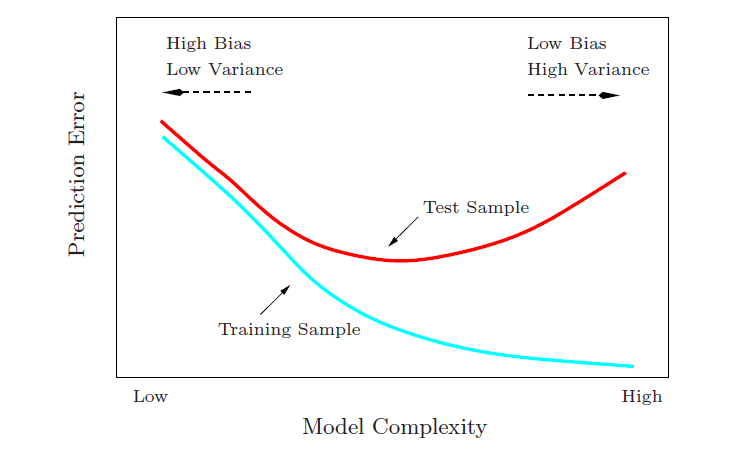
\includegraphics[scale=0.65]{Documentos Extra/Imagenes/Bias-Variance-Tradeoff.png}
\caption{Balance sesgo varianza, \cite{Hastie 2001}}
\label{fig:Balance-sesgo-varianza}
\end{figure}
 
\noindent En la figura \ref{fig:Balance-sesgo-varianza} se muestra lo que sucede cuando un modelo está en una situación de infraajuste (izquierda) o sobreajuste (derecha). En el caso de infraajuste, el modelo no se ajusta adecuadamente a los datos, ya sea para muestras dentro del conjunto de datos o para nuevas muestras que no están en los datos. Por otro lado, en el caso de sobreajuste, el modelo se ajusta demasiado a los datos recopilados y pierde capacidad predictiva para nuevos datos. Esto puede ocurrir cuando la complejidad del modelo es demasiado alta en comparación con la cantidad de muestras disponibles. 

\noindent Como hemos dicho antes, el crecimiento de los árboles tanto de regresión como de clasificación tiende a  sobreajustarse. En la siguiente parte veremos como hay distintos algoritmos que buscan evitar dicho sobreajuste. 

\newpage
\subsection{Algoritmo Random Forest}

\noindent El término bosque aleatorio se puede referir a dos conceptos distintos, uno el hecho de utilizar varios árboles sin importar como se obtienen y luego utilizar la media de los resultados o el voto por mayoría dependiendo del tipo de variable respuesta sea discreta o continua. 

\noindent El término \emph{random forest} se refiere al algoritmo de Breiman  \cite{Breiman 2001}. Este tipo de algoritmo si hace hincapié en el  método con el se construyen los árboles. También da las bases de por qué utiliza este tipo de algoritmos en \cite{Breiman 1996}.

\noindent El proceso de construcción y de utilización de los \emph{random forest} lo detallan Biau,  Scornet, y Breiman \cite{Biau 2016,Breiman 2004a} :
\begin{itemize}
\item En cada árbol se utiliza una muestra aleatoria sin reemplazamiento del conjunto de datos iniciales. La razón es buscar una muestra \emph{bootstrap} de los datos iniciales (Véase \cite{Hesterberg 2011} para más detalles de la técnica.)
\item Se establece un número $j_{try}$ por el usuario. Para cada partición a realizar se escogen de manera aleatoria $j_{try}$ variables y se elige la que más se ajusta al criterio dado. Y se hace crecer el árbol hasta que en cada nodo hoja tiene únicamente una sola observación o hasta un criterio dado por el usuario. 
 
\item Una vez se obtienen los distintos árboles del tamaño adecuado, se toma como predicción de una nueva observación la media de las predicciones de los datos en el caso de que la variable respuesta sea continua. En el caso contrario, se toma el voto por mayoría, es decir se toma la categoría o clase que mayor frecuencia tenga en todos los árboles. 
\end{itemize}

\noindent Breiman detalla las propiedades básicas de un \emph{random forest}  \cite {Breiman 2004a}. Entre estas propiedades se encuentran el sesgo, la varianza y sus acotaciones. Además Biau  y Scornet desarrollan de manera detallada las distintas propiedades de un tipo específico de \emph{random forests} \cite{Biau 2016}.

